%!TEX root = ../report.tex
\begin{document}
	\chapter{Background}
	
	\section{Natural Language Processing}
	
	Natural Language Processing evolved as a branch of artificial intelligence by combining fields such as computer science and linguistics. It helps machines to comprehend, manipulate and generate human language. Natural language processing gained interest as it seemed promising in various tasks such as human-machine interaction / communication, machine translation, spam detection, voice controlled devices, summarizing texts, and question answering in search engines \cite{nlp_appli}. Thanks to the availability of a large number of unstructured data that is created everyday (for eg. social media and medical records), efficient algorithms and powerful computing systems, a lot of advancements have been made in this field in the last few decades. 
	
	Though natural language processing is an exciting field which enables everyone to communicate with the computers in their own language (as opposed to the programming language or low level language used by the computer), understanding and making sense of human language has many layers of difficulty. The complex and diverse nature of human language, unique sets of rules and grammars for different languages, new meaning of words, different meanings for the same word, and abbreviations restrict the ability of computers to make sense of natural language. Humans have the capability of understanding, communicating, and construing very elaborate and subtle meanings, but formally defining the rules that govern the language is still a challenge for them \cite{goldberg2017neural}. This hinders the capability of taking a rule-based approach towards natural language understanding by computers as rules differ for every language and word ambiguations is commonplace. 
	
	Many Natural Language Processing tools and methods are used to bring the natural language into a format which could be made sense by computers. These techniques enable computational methods to manipulate data and make inferences from them such as how similar two sentences are, whether one sentence could be infered from another sentence, and determining the topic of an article. The most prominent NLP methods and tools are discussed below. 
	
	\subsection{Pre-processing methods in NLP}
	
	Pre-processing the text helps in bringing the input data into a form which could be digested by the algorithm. While such methods would help in computational methods, it is important to note that some of the details could be lost from the original input and the key idea is to know the pros and cons of each of these methods and to apply them where necessary.
	
	\subsubsection{Tokenization}
	
	Tokenization is a process of text segmentation which helps in splitting the text into sentences or sentences into words. Such sentences or words are called as 'tokens'. Common ways of doing this include splitting on whitespaces and splitting on punctuations. However, splitting a sentence based on whitespace or punctuations is not a straightforward task as complex words need careful attention while splitting them; e.g. "Los Angeles", "Mr. Mercedes", "i.e.", "Simon's cat", "on-campus housing" etc. To deal with such cases, rule-based or machine learning approached could be applied \cite{jurafsky2014speech}.
	
	\subsubsection{Normalization}
	
	This method is utilized to bring all text into the same format so that manipulating them would be less biased and uniform across different forms of sentences and phrases. Simple tasks such as removing punctuations, converting numbers into their word forms, and converting all text to lowercase help in putting all the data on equal footing. Though these methods sound easy, attention must be given to minute details; e.g. converting "US" to "us" does not give the same meaning. Normalization in NLP is equivalent to normalizing all the image pixels in a computer vision task so that the algorithm doesn't give importance to more colorful or vibrant images. Other normalizing methods that are used in this report includes stemming and lemmatization. 
	
	\subsubsection{Stemming and Lemmatization}
	
	These words convert the words into their base or common form. Stemming does this by "dropping unnecessary characters, suffixes, prefixes, infixes, and circumfixes from a word in order to obtain a word stem" as mentioned in \cite{kdnuggets_preprocessing}. The results of stemming could be used to find relationships and similarities between large text documents. An example of stemming could be seen as follows.
	
	\vspace{2mm}
	
	input = "I started studying yesterday"
	
	output = "I start studi yesterday"
	
	Lemmatization converts the words to the base form after going through the vocabulary and doing a morphological analysis like part-of-speech of every word \cite{jurafsky2014speech}. Lemmatization can produce better results by utilizing WordNet's lexical database of English. It offers more accuracy at the cost of time as it is an intensive and slower process. Stemming is more useful where simple database queries are carried out and time is an important factor, while lemmatization could be used for more complex tasks such as sentiment analysis.
	
	\subsubsection{Stop words removal} 
	
	Stop words should be filtered out before processing the text further as they occur more frequently in text and contribute little to the overall meaning of it while serving the purpose of connecting different parts of a sentence. Some of the most common stop words in English include "the", "so", "and", "it", and "a" \cite{nltk_list}. As can be seen from the following example, stop word removal does not change the overall meaning much. 
	
	\vspace{2mm}
	
	input = "The player hits the ball over the fence"
	
	output = "player hits ball over fence"
	
	\subsection{Bag-of-Words}
	
	Machine learning algorithms often require structured inputs of fixed lengths. This is one of the major issues in feeding the text into a machine learning model. Text must be converted into numbers or vectors in order to use them in the algorithms. Constructing vectors out of text is called as feature extraction or feature encoding. Bag-of-words in one such simple technique of converting text into vectors of fixed length.
	
	Bag-of-words captures the count of each unique word in a text. It is made up of a collection of unique words and a measure of occurrence of those words in the document. This technique simply bags same words ignoring the order and structure of the words in the text. Bag-of-words works well for topic modeling (determining the topics that occur in a collection of text) and text classification since the intuition behind this is that similar documents mostly share the same words \cite{bow_model}.   
	
	An example of Bag-of-words model:
	
	Consider each of the following lines as a single text document.
	
	"The boy fell from the tree" \\
	
	"The boy fell from the tall tree" \\
	
	"The kid climbed the tree" \\
	
	"The girl is sick" \\
	
	The unique words in all of these texts after converting them to lowercase would be;
	
	"the" 
	
	"boy"
	
	"fell"
	
	"from"
	
	"tree"
	
	"tall"
	
	"kid"
	
	"climbed" 
	
	"girl"
	
	"is"
	
	"sick"
	
	In order to convert the first text into a vector, these unique words are stacked in a row and the number of occurrence of each of these words in the text is represented as a number in the box indexed by the corresponding word. This results in a vector of length 11. Fig \ref{bowex1} shows how this is done. 
	
	\begin{figure}[h!]
		\centering
		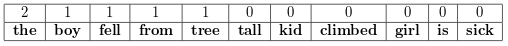
\includegraphics[scale=0.5]{images/bowex1}
		\caption{Vector representation of the first sentence.}
		\label{bowex1}
	\end{figure}
	
	Similarly, all other texts are converted into a vector of same length as shown in Fig \ref{bowex2}.
	
	\begin{figure}[h!]
		\centering
		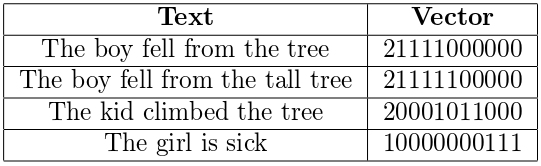
\includegraphics[scale=0.5]{images/bowex2}
		\caption{Vector representation of all the sentences.}
		\label{bowex2}
	\end{figure}
	
	It can be seen that the first three texts are closer to each other in the vector representation and the last sentence is significantly different from the first three. Such a representation is very consistent in extracting features from new documents and can scale to larger texts. However, when using a large corpora, the vectors might get sparse due to very few known words in the vocabulary and many new words that get ignored in the vector representation. This ends up in a large sparse matrix which demands more computational power and memory. Techniques such as ignoring frequent words, stemming the words to their root form, correcting the misspelled words and grouping similar words could be used to reduce the size of the sparse matrix \cite{bow_model}.
	
	Though the bag-of-words model is very simple to interpret and very flexible, it has few limitations such as;
	
	\begin{enumerate}
		\item Vocabulary - The words to be included in the vocabulary, which in turn directly affects the vectorization of text and the size of the sparse matrix, should be designed and chosen carefully.
		\item Sparsity - The sparse representation of Bag-of-words model contributes to the high space and time complexity. The models are forced to infer knowledge from a very large representation which is quite cumbersome. This should be taken care of while modeling the matrix in such a way that it is as less sparse as possible.
		\item Meaning - The semantics of the text is ignored in the bag-of-words model as the order of the words are not considered. Thus, the distinct meaning of texts with the same words arranged in different order will not be captured by this model. 
		
	\end{enumerate}     
	
	
	\subsection{Term Frequency - Inverse Document Frequency (tf-idf)}
	
	Tf-idf is a statistical tool to determine "how important a word is to a document in a collection or corpus" \cite{tf_idf_defi}. Tf-idf is used widely to weight important terms in applications such as text-based recommendation systems, document classification and information retrieval. It captures the most important words in a document by combining two algorithms, namely, term frequency and inverse document frequency.
	
	\begin{itemize}
		\item Term frequency - This captures the number of occurrence of a word in a document. To consider the length of the document while calculating the term frequency, the frequency of the words is divided by the total number of words in the document. The term frequency of a word $t$ in a document $d$ is defined as mentioned in \cite{tf_idf_1};
		
		\begin{equation} tf(t,d) = \frac{\text{number of occurences of term in the document}}{\text{total number of all words in the document}} \end{equation} 
		
		\item Inverse document frequency - Words like "the" occur a large number of times in most of the documents and these words get more score in the term frequency calculation. However, such words have very less amount of information for most of the tasks. Hence, it is preferable to assign a lower score to these common words which contain no information. Inverse document frequency achieves this by calculating a low score to frequently occurring words and increasing the weights of the words that occur rarely. Inverse document frequency for a word $t$ in a document $d$ is defined as mentioned in \cite{tf_idf_1}. 
		
		\begin{equation} 
		idf(t) = \frac{\text{total number of documents in the corpus}}{\text{number of documents with term t}} 
		\end{equation}
		    
	\end{itemize} 
	
	The tf-tdf score of the term $t$ and document $d$ is calculated as;
	
	\begin{equation} tf-tdf(t,d) = tf(t,d) \times idf(t) \end{equation} 
	
	Words which have a very high term frequency and low document frequency among the collection of documents, thus capturing the important and rare unique words pertinent to the task \cite{tf_idf_defi}. 
	
	
	
	\subsection{Word Embedding}
	
	Word embedding is a NLP task which converts text into an array of numbers or real valued vectors. Such a representation of words proved to be useful in many tasks such as semantic similarity measures, text classification, and machine translation. Though one-hot-encoding (where a sentence is represented by a matrix with its dimension equal to the number of words in the sentence and each row made up of 0's with a 1 in the dimension corresponding to the word) was used in the beginning as a word embedding model, it has issues such as being a sparse matrix, redundant memory, and inability to capture the context or the relationship between different words in the same sentence. 
	
	More compact and meaningful representations of words evolved later with the use of neural networks and a large corpora to learn the distributions of words on. The most popular algorithms which exist today for efficient word embedding include Google's Word2Vec \cite{word2vec}, Facebook's fasttext \cite{fasttext}, and Stanford's GloVe \cite{glove}. These algorithms were able to capture both the semantic relationships and context of each word and represent them in a more compact way (dense vectors) \cite{shane_wordembedding}. Fig \ref{simple_embedding} below depicts a 2D representation of word embeddings where similar words in context and meaning have been grouped together in the vector space. 
	
	\begin{figure}[h!]
		\centering
		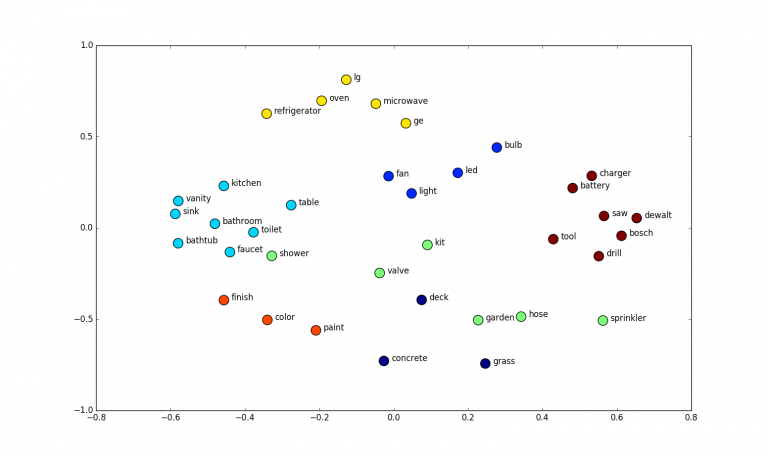
\includegraphics[scale=0.5]{images/2d_word_embedding}
		\caption{Example 2D word embedding space, where similar words are found in similar locations. Image from \cite{2d_embedding}.}
		\label{simple_embedding}
	\end{figure}
	
	\subsection{Part of Speech(POS) tagging}
	
	Same words give different meaning when they occur in different positions of the sentence. The context and the order of words are very important in determining the semantic meaning of a sentence. Bag-of-words and tf-idf do not capture such differences and consider the same words without any regard to their placement. The meaning of the word "address" in "May I have your address?" and in "I had to address to the public" is different. Hence, the position and context of the word in every sentence is imperative to capture the sematics of it. 
	
	Part-of-speech of a word is the function of that word in a sentence. Commonly seen parts of speech include nouns, verbs, adverbs and adjectives. In computational linguistics, such tags are determined based on factors such as its definition, context, its neighboring words and its relationship with them \cite{pos_wiki}. 
	
	\begin{figure}[h!]
		\centering
		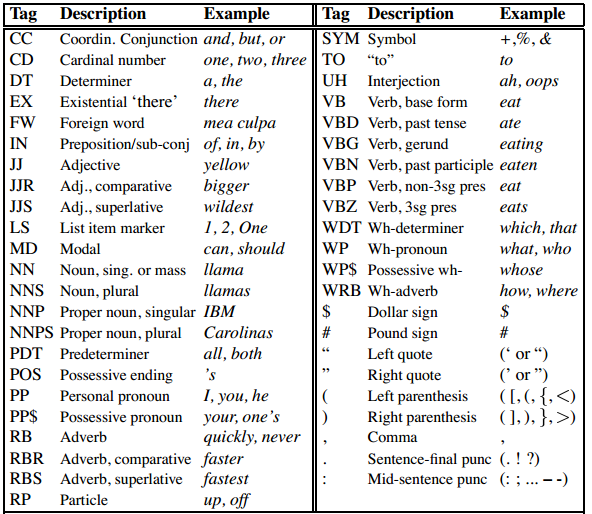
\includegraphics[scale=0.6]{images/penntagset}
		\caption{Penn Treebank part-of-speech tags. Image from \cite{jurafsky2014speech}.}
		\label{penntagset}
	\end{figure}
	
	
	Determining the part of speech of every word in a sentence is imperative to many applications of NLP. Tasks such as text to speech and word sense disambiguation require POS tagging a pre-requisite to achieve better performance. In order to stress the words in line with their semantic interpretation, text to speech application needs to know the function of each word in the sentence. Similarly, word sense disambiguation makes use of POS tags to find out the sense in which a word, which has multiple meanings, has been used in a sentence. Rule-based tagging, statistical methods which use Hidden Markov Models, and memory based tagging are some examples of computational algorithms which are used for assigning parts-of-speech. Penn Treebank tagset is one of the most popular tagset used in the modern language processing algorithms \cite{jurafsky2014speech}. Fig \ref{penntagset} shows the list of 45 POS tags that are included in the Penn Treebank tagset.
	
	\subsection{Named Entity Recognition (NER)}
	
	It is often the case that detecting the real world entities in text makes information extraction easier. Named entity recognition is such a technique which goes through the entire text, extracts keywords (nouns) and maps them to pre-defined categories of real world entities such as locations, companies, cities, organization, dates, and individuals. For e.g., an unannotated text "Microsoft was flourishing in business when Barack Obama was the president of the United States." would be annotated by a named entity recognition algorithm as follows; \\
	
	\{"Microsoft": Group, "Barack Obama": Name, "United States": Place\} \\
	
	NER facilitates many real world applications. Classifying and managing a large news database is very time-consuming and error prone when it is done manually. Instead, a NER algorithm can swiftly extract the important entities such as names, locations and organizations mentioned in each article and group them in a hierarchical order using the tags. This ordering could be used for efficient retrieval and categorization of the articles. Optimized search algorithms use NER to concentrate on the keywords for searching rather than the naive method of going through the whole text. Recommendation systems in news and other blog websites implement NER to capture the organizations, places and individuals each reader is interested in and recommend similar news articles or blogs to them. Thus, structuring and categorizing a large unannotated text using NER could be facilitating faster language processing for more complicated inferences \cite{ner_blog}.
	
	\subsection{Dependency Parsing}
	
	All the techniques which have been described above work in the syntactic level. A lot of information about the context is lost when a task is designed to only take into account the syntactic properties of documents. Such techniques fail in the case when the words have more disambiguation with multiple meanings. Processing those words in a semantic level would help build a more meaningful and accurate description of a sentence. Dependency parsing helps in sentence level disambiguation by eliciting grammatical relationship between words in a sentence. Based on the verbs, it tries to find out the relationship between the other nouns, adverbs and adjectives in the form of a head-dependent or parent-child format. For e.g., the result of parsing the sentence "Mary laid the mug on the table" using spaCy library's dependency parser is shown in Fig \ref{deptree}
	
	\begin{figure}[h!]
		\centering
		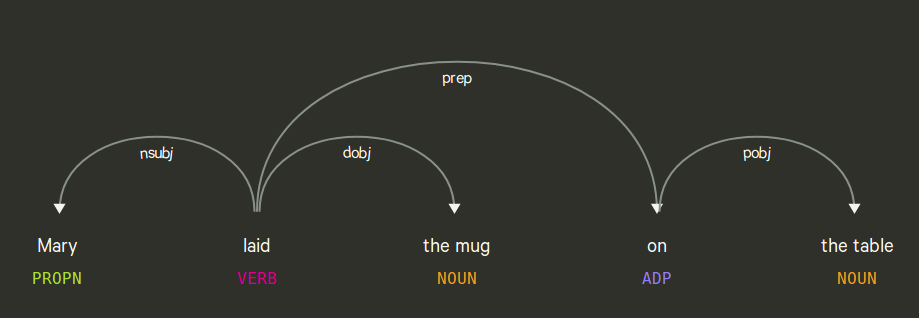
\includegraphics[scale=0.3]{images/deptree}
		\caption{Dependency parsing of a sentence using spaCy library \cite{dep_visi}.}
		\label{deptree}
	\end{figure}
	   
	As can be seen from Fig \ref{deptree}, it could be easily inferred that "Mary" is the subject (denoted as "nsubj") and "the mug" is the object (denoted as "dobj") of the verb "laid". Parsing in this manner is utilized for question answering systems and in grammar checking tools. nominal subject(nsubj), clausal subject(csubj), direct object(dobj), indirect object(iobj), determiner(det), prepositional modifier(prep), and object of preposition(pobj) are some of the grammatical relations found in dependency parsing \cite{de2008stanford}.
\end{document}